% Maintain the consistency.
% Maintain a good writing flow. 

\section{Introduction}\label{sec:introduction}
One of the most significant advantages of employing technologies is that, in most circumstances, it is less expensive in terms of time and instantaneous time in most of the cases to do the same task than it would be with an analog process. Conventionally, we continue to do all of the official activities via the use of paper documents. In addition to increasing time consumption, it also makes students more reliant on authority and the particular time limits impose by the authorities. Furthermore, there is always the possibility of being unsuccessful in finishing the procedure, whether or not the information is incorrect. In addition, manually recording attendance is a time-consuming process that takes a long time. Our objective is to create an application that will transfer these two procedures to a digital platform, which will, of course, be able to complete the duties in the shortest amount of time imaginable and with the least amount of paper work possible. The system should be able to provide students with the independence from the tormenting limits of the administration while also allowing the authorities to make their responsibilities more manageable for themselves. For both students and administrators, it goes without saying that the program would be user-friendly in its design.

This document is a record of a strategic and creative process that was focused on clearly describing concerns and objectives, as well as providing an overview of the application that represented the narrative from the beginning to the completion of the process. Anyone interested in using or developing the system would be able to do so with the assistance of this documentation.

The purpose of this course is to develop a database application system by applying the theories, methodologies, tools, and technologies we learnt in CSE 413 that is Database System course.  

\clearpage


\subsection{Background and Motivation}\label{subsec:bm}

Every year since the university's founding in 1966, the number of students has increased by a small but steady margin. Despite the fact that the globe is being exposed to new technology on a daily basis, the method for receiving fees and the attendance system at the University of Chittagong have stayed the same. This is due to the fact that it is reliant on a single branch of a single bank, making the payment system for tuition difficult to manage not just for students but also for the administration. Students despise this analog approach, especially since they are restricted to a one-day time frame to deposit the money during class days or in the weeks leading up to the test. As the number of students continues to rise at a good pace year after year, it seems that university administrators, as well as bank administrators, have had enough of this terrible procedure. The same may be said regarding the old method of attendance. Teachers have been seen to devote 25 to 30 percentile of a class period to attesting attendance in the traditional manner.

If we take a closer look, we will see that these issues are interconnected. We want to create a system that can tackle these difficulties while also processing some basic data from both students and instructors. To accomplish the functions, the system will not need any paper work and will demand the least amount of physical presence from authorities as well as students. Throughout the development of the application, both the payment and attendance systems will become one-click operations. The capability for administrations to query the necessary information will be more accessible than ever before. Students and administrators may use this program to run processes from any location at any time, with an immediate time stamp to validate it.

\subsection{Problem Statement}\label{subsec:ps} 

\emph{To develop a database system that can be used to handle payment system of fees of student and attendance system online.}

The system will be using student data such as \emph{name}, \emph{student id}, some institutional data such as \emph{course}, \emph{department}, some teacher's data such as \emph{teacher's name}, \emph{the department he belongs to} and \emph{which courses he teaches} and so on. The system will also hold the records of payments already done or have to be done by a student. With the information of courses from a teacher and the students studying the course, the attendance system will be implemented in the same application.

\clearpage

\subsection{System Definition}\label{subsec:sd} 

\textit{``An online application that is used to manage the payment system for fees by students as well as the attendance system for such students. Transforming and shifting the analog payment system to a digital platform should be accomplished via the application, avoiding the time-consuming approach."}


\subsection{System Development Process}\label{subsec:sdp}

A process known as the software development life cycle is divided into various parts (SDLC). The requirements collection and analysis step is the most critical element of the whole process. It is at this phase that the client explains his or her expectations for the project, including who will use the product, how the customer will use the product, and the specific data that will be included with any unusual client needs that have been recognized. Project managers often use a variety of approaches to gather the requirements for their projects. Interviews, surveys, observations, and workshops are some of the most well-known types of research methods. We employed interview and questionnaire methodologies to gather the requirements because we were determined to do so.\\

\begin{figure}[H]
    \centering
    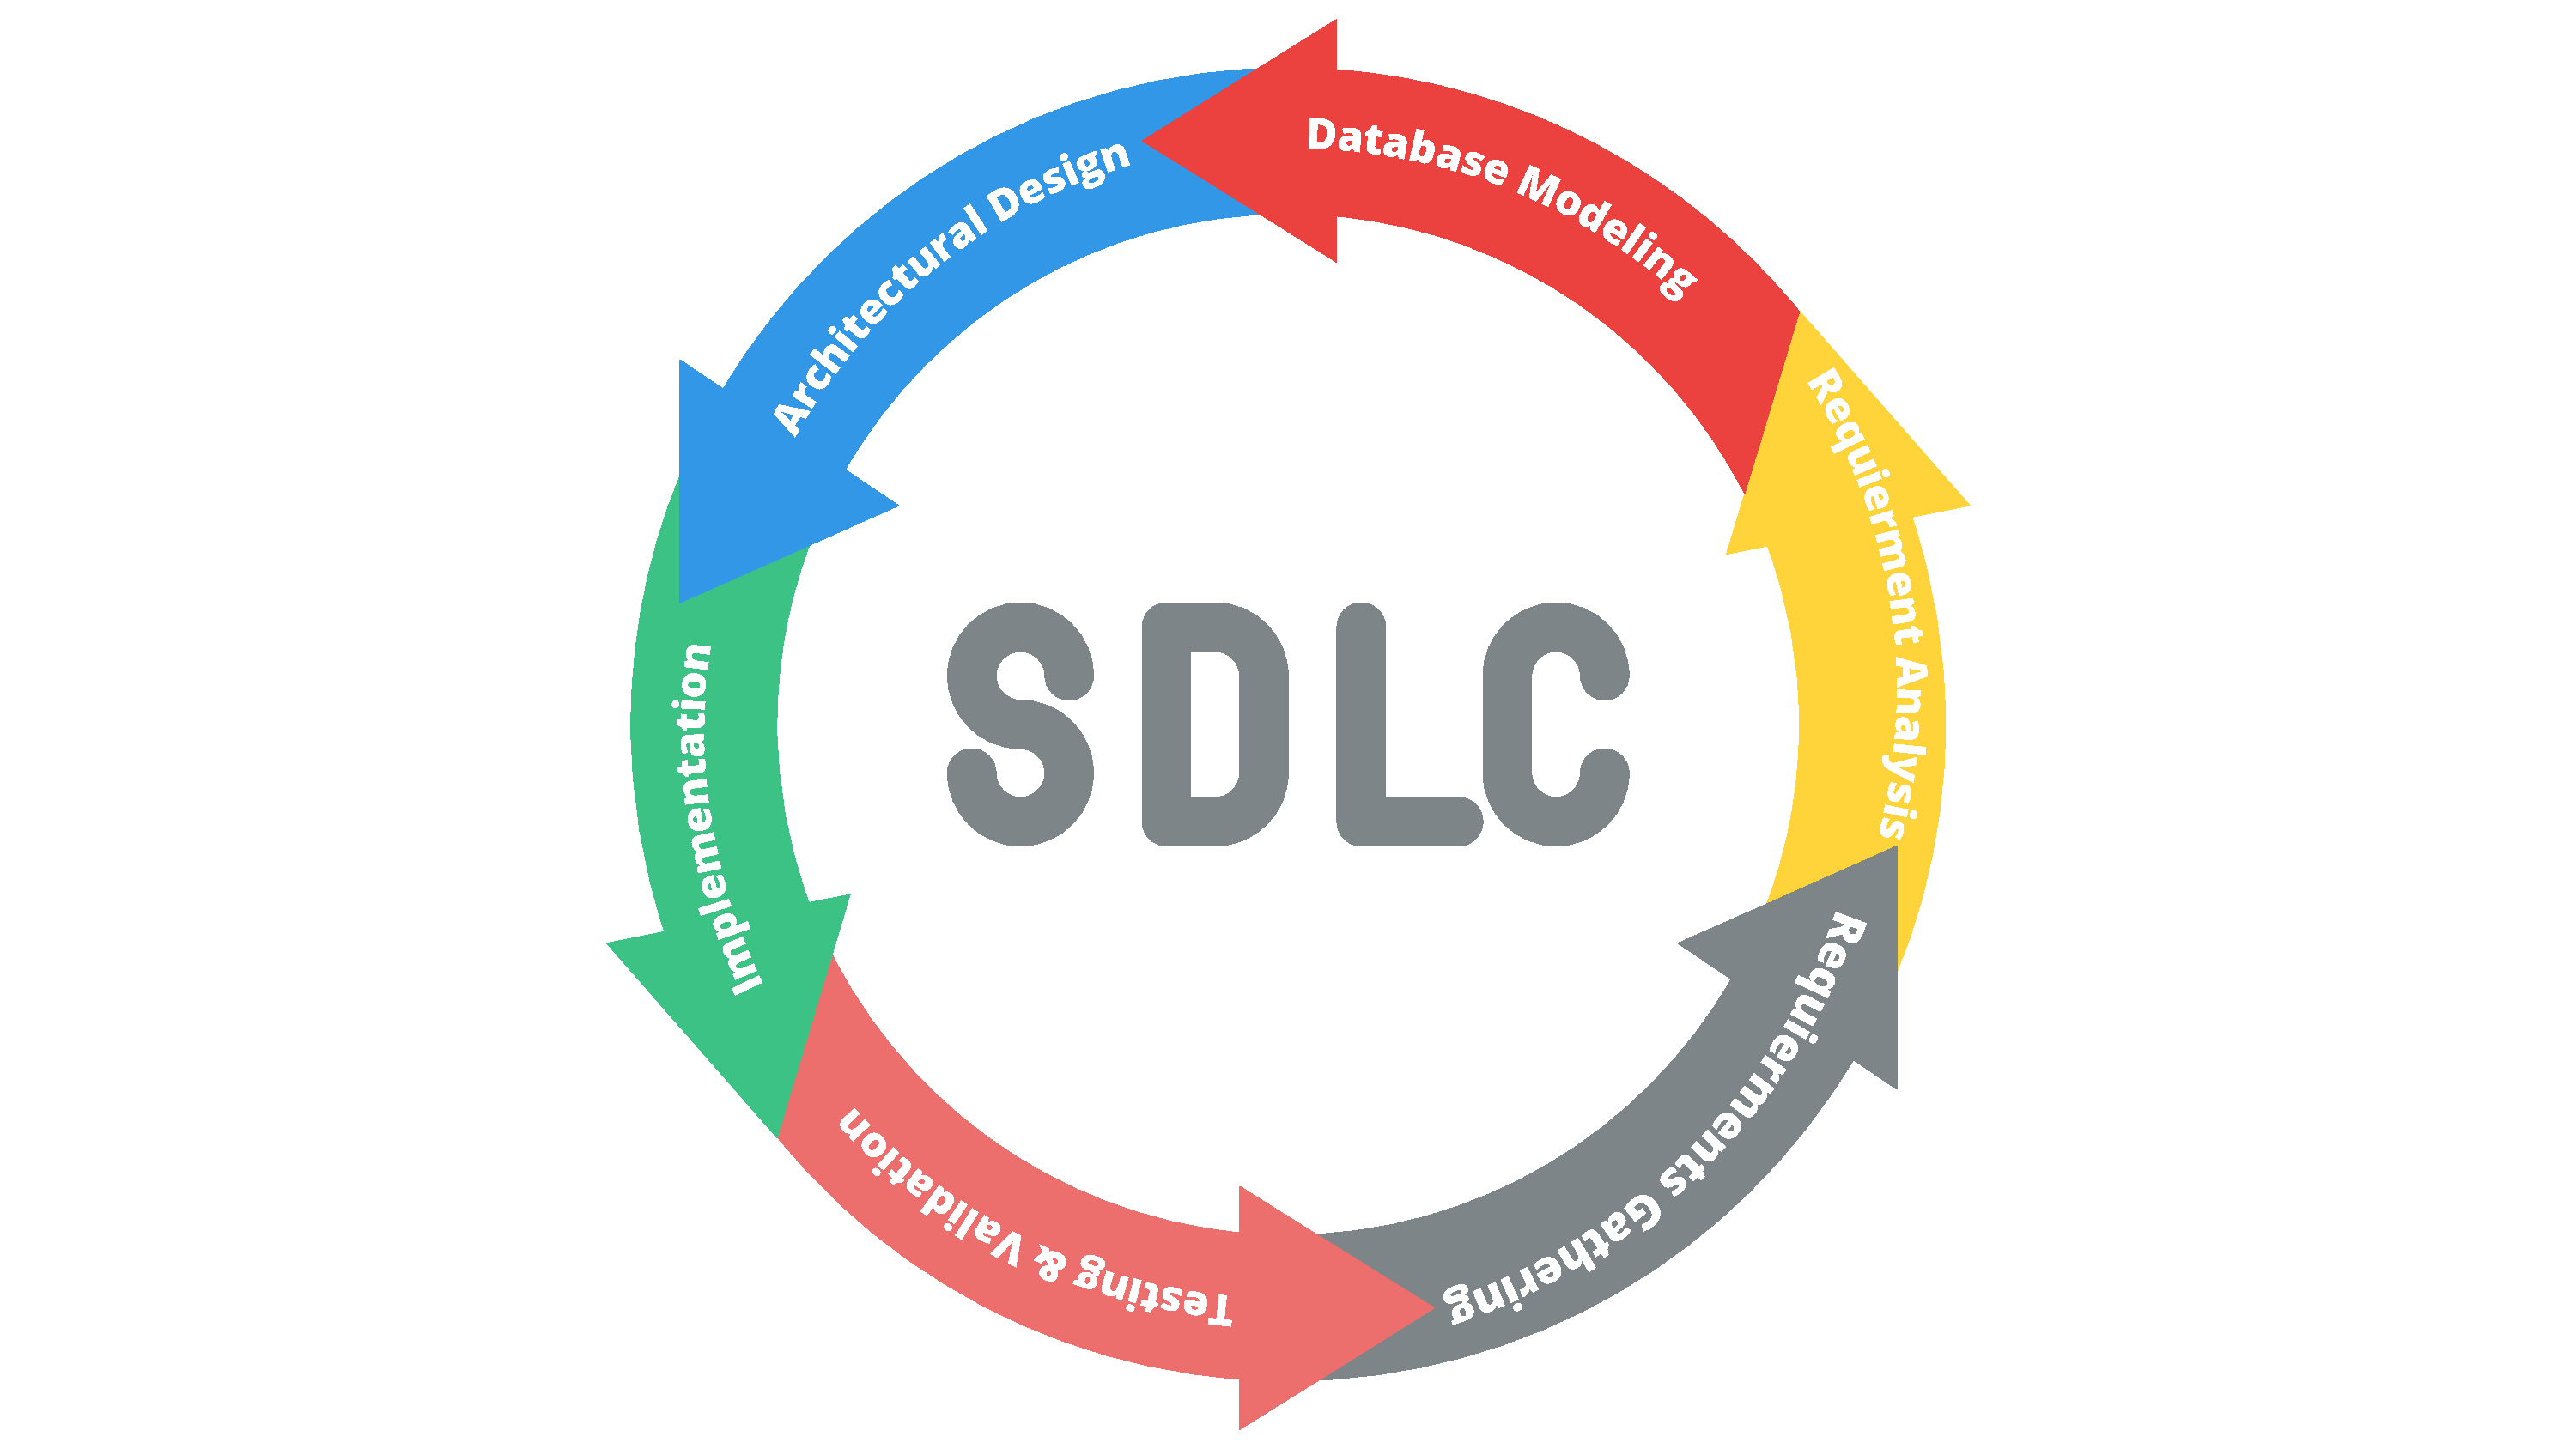
\includegraphics[width=1\textwidth]{images/sdlc}
    \caption{Software Developement Life Cycle (SDLC)}
    \label{fig:sdlc}
\end{figure}

The research of requirements is vital, as is the basic movement that occurs once the requirements are gathered. We disassemble, improve, and study the needs that have been gathered in order to generate predictable and clear requirements. As part of this effort, all requirements are audited and a graphical view on the whole framework is provided. Afterwards, when the assessment has been completed, it is common for the task's understandability to significantly increase in terms of comprehension. In this case, we may also make use of the client's relationship to describe areas of disarray and determine which needs are of more importance than others.\\

When it comes to database modeling, it's also referred to as data modeling since it involves establishing a data model for the data that will be kept in the database. The third phase of the SDLC is known as the design phase. This data model is a conceptual representation of data items, the connections that exist between them, and the rules that govern them. The Data Model is defined as a theoretical model that organizes information representation, information semantics, and consistency limits of the information in a way that is understandable to the user. The information model emphasizes what information is necessary and how it should be organized, rather than what actions will be done on it, as opposed to the tasks themselves..\\

There are basically three types of data models. These are conceptual data models, logical data models, and physical data models,  each with a specific purpose.\\

\begin{itemize}
  \item The conceptual data model mainly defines what the system contains. This model is commonly created by business stakeholders and Data Architects. The intention is to put together, scope, and characterize business ideas and rules.
  \item The logical data model defines how the system should be implemented independently of the DBMS. This model is regularly made by Data Architects and Business Analysts. The object is to foster a specialized guide of rules and information structures.
  \item The physical data model depicts how the system gonna be implemented using a particular DBMS. This model is commonly made by DBA and engineers. The intention is the actual implementation of the database.
\end{itemize}

A system architecture is a representation of the structure of a system that is intended to be used as an illustration. It encompasses all of the system's components, as well as subsystems that handle all of the system's operations in their entirety. CU-OPAS is a web-based application system that uses request-response patterns to communicate with users. Any legitimate user of this system may request inquiries about payment and attendance activities from the backend API by using the frontend user interface on the system's front end. After that, the backend API communicates with the database server and creates a response in response to the queries that are provided back to the frontend application.\\

\begin{figure}[H]
    \centering
    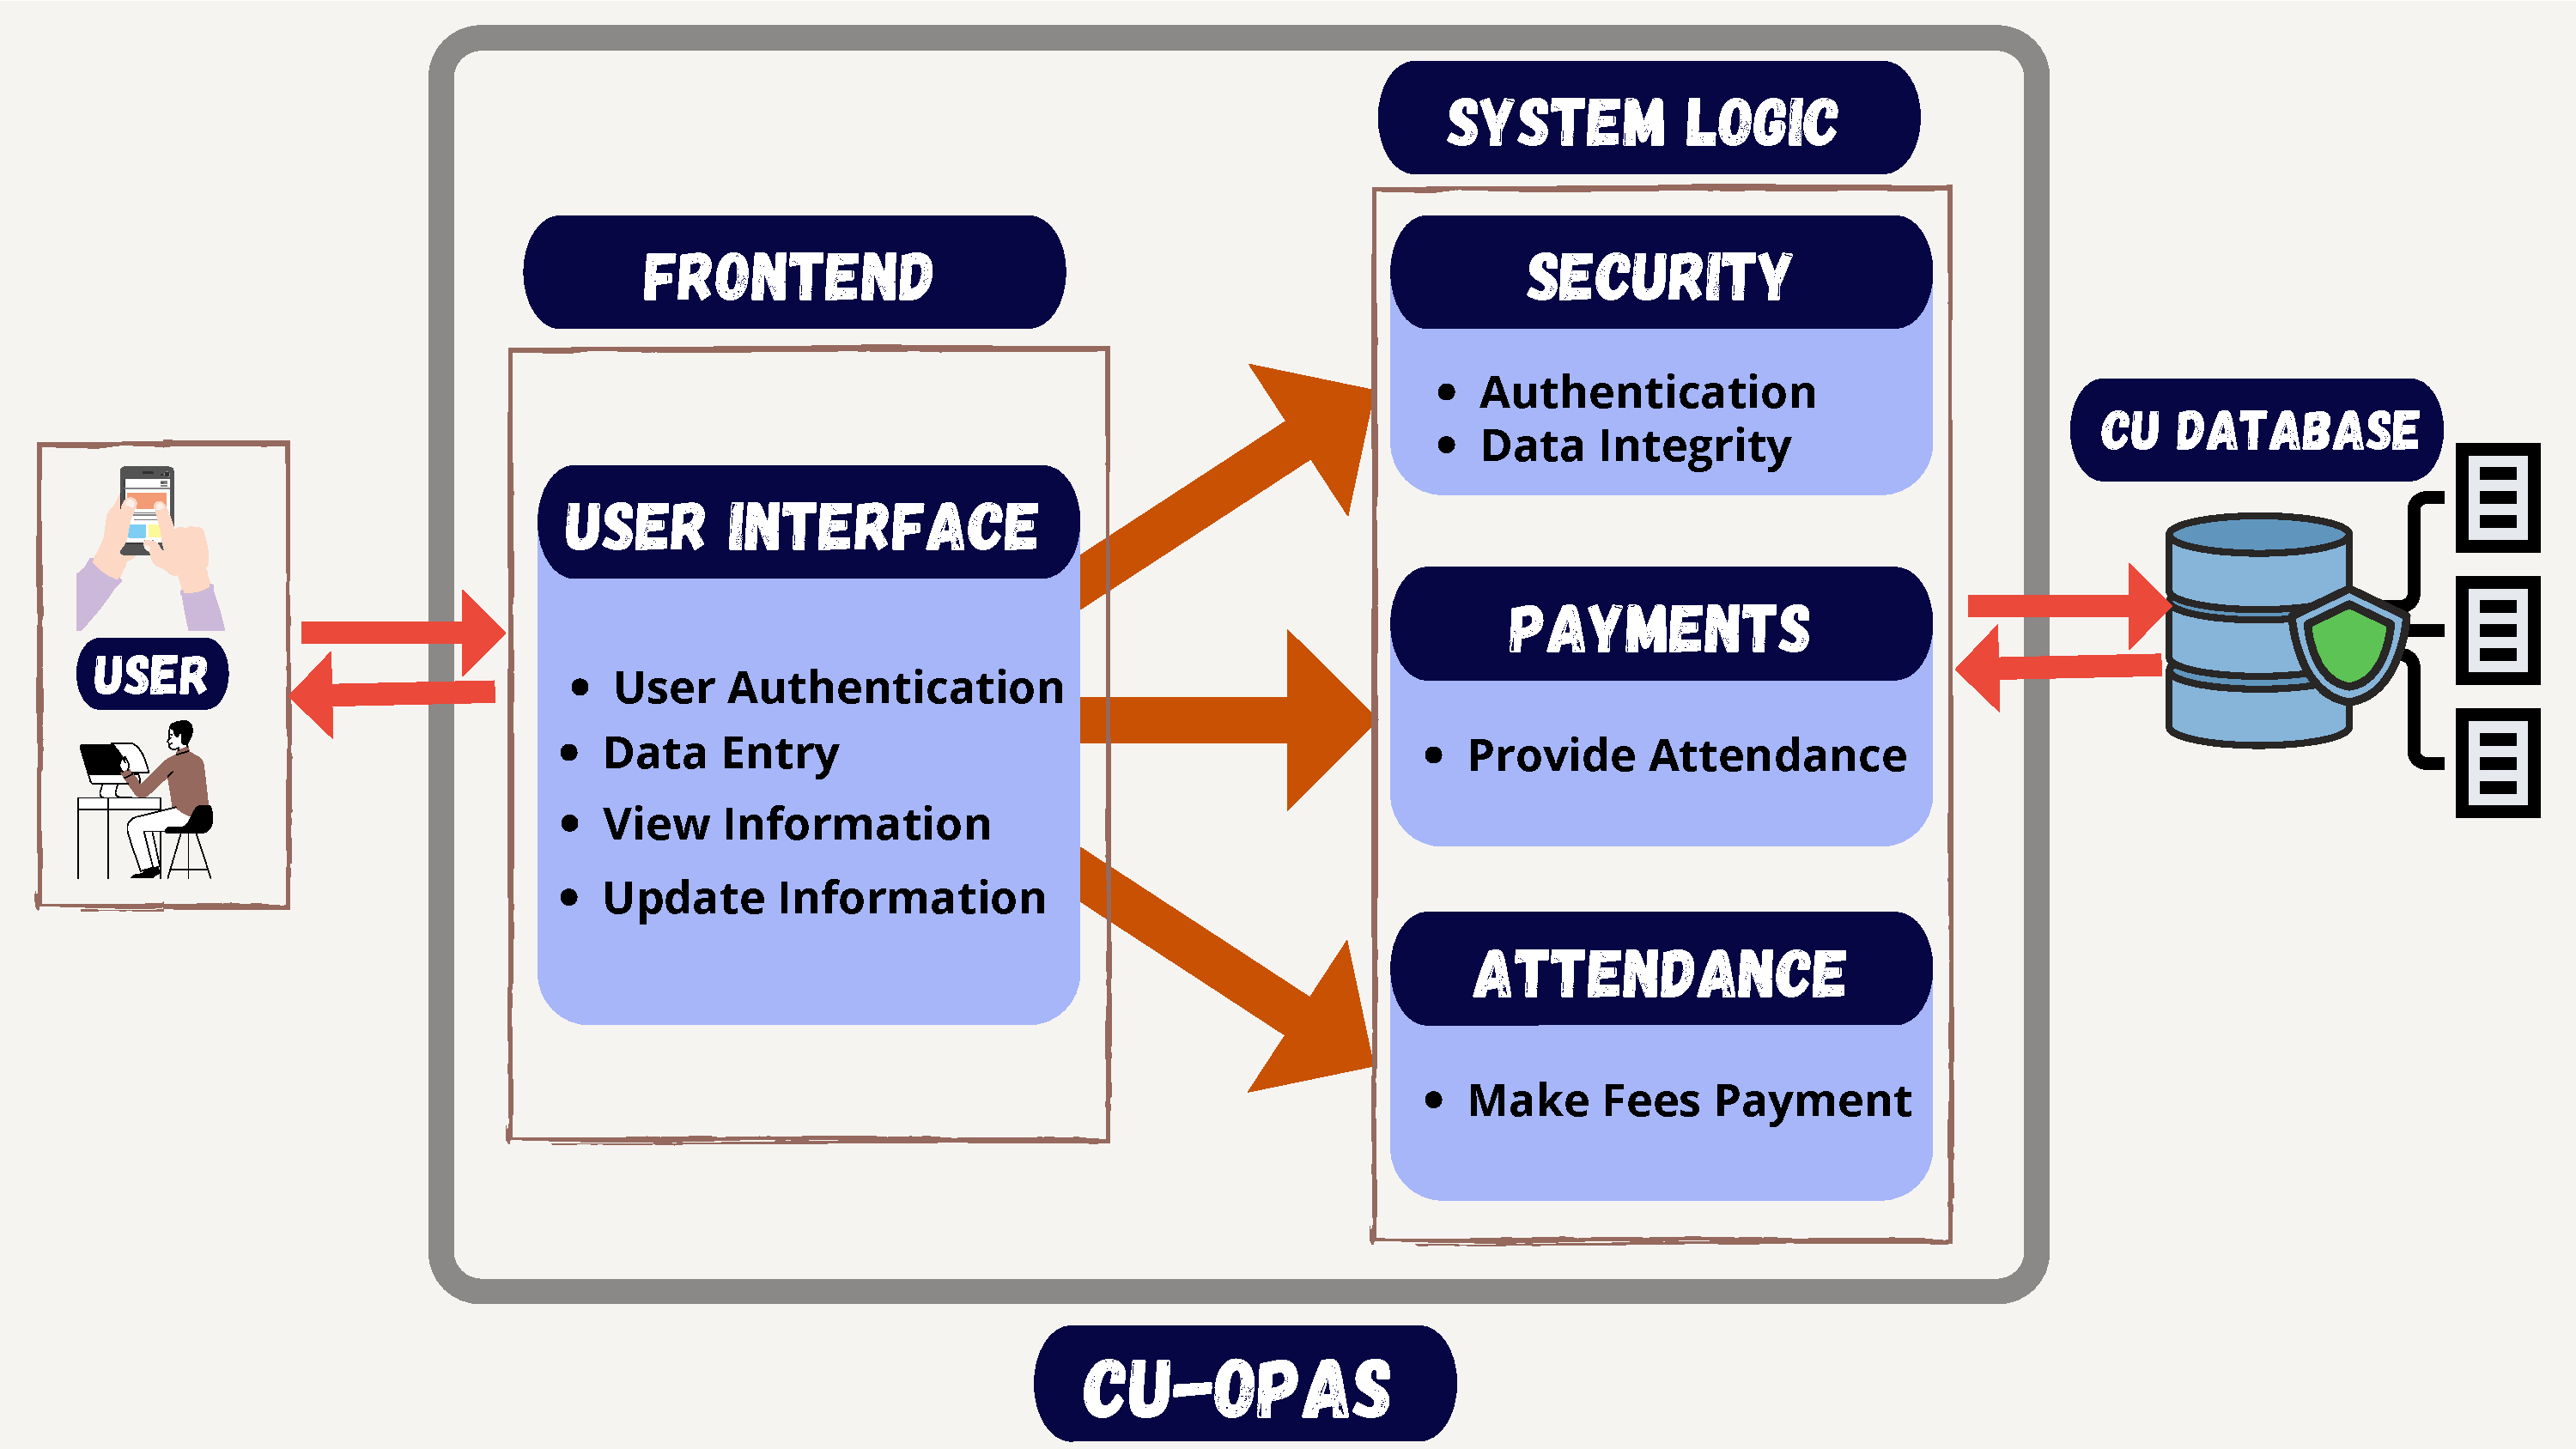
\includegraphics[width=1\textwidth]{images/archi}
    \caption{Architectural design of CU-OPAS}
    \label{fig:archi}
\end{figure}

The implementation process starts when the architectural design and user testing have been completed successfully. It is at this phase when the physical design of the system is completed. It is the third phase of the SDLC. As part of this phase, we employed a range of programming languages, frameworks, tools, and online resources to construct our system from scratch.\\

The final and most crucial phase of the SDLC is validation. This step is critical in ensuring that not just the proper product, but also a high-quality product is produced. Validation can determine whether or not the system meets end-user requirements. We've tested our system in a variety of ways for this aim, including Unit Testing, Integration Testing, System Testing, and Acceptance Testing.
\begin{comment}


To design a database, one should follow the following steps:
\begin{enumerate}
\item Requirement analysis
	\begin{itemize}
		\item[-] interviewing, documentation, etc .
	\end{itemize}

\item Mapping onto a conceptual model (conceptual design)
     \begin{itemize}
     	\item[-] ER model
     \end{itemize}
\item Mapping onto a data model (logical design)
	\begin{itemize}
     	\item[-] Relational model, object model etc. 
     \end{itemize}
\item Normalization
\item System Architecture
\item Realization and Implementation (physical design)    
    
\end{enumerate}
\end{comment}


\subsection{Organization}
Section~\ref{sec:introduction} gives an overview of this project. this section also narrates the project from start to the end briefly. Section~\ref{sec:projectmanagement} describes how the project and the resources are managed. The next section~\ref{sec:rga} refers to the results of the analysis of the information gathered from the surveys, interviews and discussion with some group of students, teachers and administrative officers. The following section~\ref{sec:cm}, section~\ref{sec:lm} and section~\ref{sec:norm} gives the overview of how we designed the database and enhanced it step by step as most as possible. Section~\ref{sec:sa} and section~\ref{sec:imp} gives the information about the whole system structure and how we implemented it. Section~\ref{sec:val} says how we validated the system with real user data with an statistics on consumed time, cost, user satisfaction between the previous system and this system. Section~\ref{sec:sd} is about the process to install and configure the system so that even a non-technical person can use the system easily. Finally, the conclusion and the pointers to the future work are outlined in Section~\ref{sec:cfw}.

\clearpage